% siminos/blog/atlas.tex
% $Author$ $Date$

% \chapter{Atlas}
% \label{chap:atlas}

\subsection{Blogging fluid dynamical thoughts}

\begin{description}

\item[2012-03-19 Predrag~~] to Daniel and Mike: this section is copied
from pipes/blog/ , written together with Marc and Ashley. If you want to
join, I'll give you access. But I will not do the secretarial work of
pasting your email in here. Ask Mr. Remolina for assistance in such
matters...

\item[2012-03-19 Predrag~~] A letter to John F Gibson, Divakar, Rich and
Johann:

This is not quite there yet, but \HREF{../slice/ACHKW11.pdf}{here it is}.

I have 3 converts to symmetry reduction; in case of pipes, it is a
necessity, because without it nothing could be done, but also Mike Schatz
is now enthusiastically slicing his 2-dimensional Landau flows.
\\
{\bf 2012-03-20 Johann}
(continuation of conversation we started in Kyoto 2008-03-20)
I later realised that the \mslices\ ('quotienting' is clearer to me)
was a very strong tool not only for identifying RPOs/TWs connections
between various exact states, but also simply as a visualisation tool.

{\bf 2012-03-20 Predrag}
Took me a while to settle on nomenclature, so please do not undo it.
Let's use 'quotienting' to mean {\em any} symmetry reduction scheme. My
2008-03-20 proposal to you is what Marsden people call 'method of
connections.' It maybe deep, but for us it is not useful, as relative
periodic orbits \emph{do not} reduce to periodic orbits in this approach
- the best thing I know of now is the method of slices. So, please use
\mslices\ is you are slicing (the word means that in mathematics since at
least 50's and French respect mathematics, no?), 'quotienting' is you are
just talking, but not actually doing anything.

Any chance of going back to plane Couette or pipe relative periodic orbits?
\\
{\bf 2012-03-20 Rich }  I'm processing the data as we speak.
\\
{\bf 2012-03-20 Johann}
At the moment I have an ongoing interaction with the KTH and Marburg
people (including two PhD students, one of which I supervise with Dan
Henningson and Philipp Schlatter) on the flow called ASBL (Asymptotic
Suction Boundary Layer). It is a parallel version of the Blasius boundary
layer flow, achieved in practice by sucking gently at the wall. It shares
all the features we like about Couette or pipe (base flow linearly stable
up to very high Re, transitional spots, etc... and it clearly has two
continuous symmetries in x and z like pCf. Our focus at the moment is more
on edge states and alike rather than the turbulent state itself. In a
small periodic box the edge state is a RPO with shifts in both x and z.
Your \mslices\ is perfectly relevant for this flow, so I
already suggested a few months ago that the students should implement a
slicing subroutine but failed so far at motivating them (you already
experienced that I presume).
\\
{\bf 2012-03-20 Predrag}
I have been working on this very hard - and have several comic-book
versions coming up. Our
\HREF{http://www.cns.gatech.edu/~predrag/courses/PHYS-7224-12/schedule.xml}
{Chaos Course} students understand most of it, and even some faculty is
starting to learn (that's a real achievement). I propose that you guys
join the
\HREF{http://www.math.gatech.edu/seminars-colloquia/series/cdsns-colloquium/predrag-cvitanovic-20120326}
{seminar} I will give on Monday 2012-03-26 at 11:00 (17:00 your time). If
you want to join, I'll make it a
\HREF{http://www.cns.gatech.edu/colloquia-seminars/AudioVisual.html}{webinar}.


{\bf 2012-03-20 Predrag}
The thing is, from my experience with (gasp!) Kuramoto-Sivashinsky, the
turbulent dynamics resides in the full state space\rf{SCD07}, and has
nothing to do with what one finds in the discrete-symmetry invariant
subspace\rf{lanCvit07}. The same for pipes - the turbulence in a
symmetric subspace has nothing to do with the turbulence in a less
symmetric space that we work with.
\\
{\bf 2012-03-20 Rich } I totally agree - physicists like symmetry more
than Nature.
\\
{\bf 2012-03-20 Johann}
What do you mean exactly by 'nothing to do'? This you should say to Genta
who is back on track with the super-symmetric periodic orbits found first
by him and Lennaert. Rich has also identified recently (APS 2011) many
periodic orbits in a 2D Kolmogorov flow.


{\bf 2012-03-20 Predrag}
Intent of this paper is pedagogical, so it is still not in the full state
space - just like in plane Couette, my collaborators have `physical'
intuition that spanwise motions are insignificant compared to the
streamwise. I doubt it - plane Coutte puffs are pretty much of equal
extent streamwise and spanwise.

\item[2011-11-15 PC~~]
I am worried about this statement - where does
    $\velRel_\theta=O(10^{-3})$ come from? We believed the same for \pCf, but
    when one goes to large aspect ratios, the `puffs' tend to be of the
    same size in the stream-wise and span-wise directions:
``This is
usually imposed by symmetry, but one could argue that it is the strong
stream-wise advection that favors structures with  ever so weak azimuthal
rotation, $\velRel_\theta=O(10^{-3})$.)''
{\bf APW 111220} I think I took this from the known cases
\rf{Pringle07}.

\item[2012-03-20 Johann~~]
Those flows all have a well-defined advection direction imposed by the
boundary conditions, so it is intuitive for everyone that the streamwise
shift (which have no reason to be commensurate with the parameter $L_x$) is
the first to get rid of. For the spanwise shifts it is more delicate to
understand what creates them. For instance in the ASBL the spanwise shift
of the edge-RPO is always exactly $L_z/2$ so it is more likely to be
associated with the discrete z-symmetries of the problem rather than the
tranlsational symmetry.

As for the 'puffs' of \pCf\ (I presume you talk about the turbulent
'stripe'), the situational is slightly different since locally there truly
is an oblique mean flow adjacent to the turbulent regions, on which I am
working at the moment.  BTW, I am much involved in simulating and
understanding the spatio-temporal aspects of subcritical transition,
interacting strongly with Paul Manneville and other Parisians. When this
is written down I'll send it to you.

Something else I started doing is a closed 2D convection flow, both the
transitional aspects and chaotic advection of tracers. My flow has no
continuous symmetries, only a discrete one. It goes periodic,
doubly-periodic then chaos with no symmetry. We did not detect Arnold's
tongues. Does someone have evidence for UPOs born right at the onset of a
Ruelle-Takens route to chaos? People like Letellier talk about toroidal
chaos and argue that looking for UPOs is pointless. So I'd like to hear
your opinion and suggestions for something to read.

\end{description}


\subsection{Blogging slicing progress}
\label{chap:atlasBlog}

\begin{description}
\item[2011-11-30 Predrag]
started a new blog, for Predrag and Chaos Gang planned paper

\texttt{siminos/atlas/atlas.tex}


\item[2010-07-07 PC]                                    \toCB
A more mathematical thing to fix (not essential if we stick to $\SOn{2}$
case): a clear discussion how the projection of the group tangent version
works for simple Lie groups of dimension higher than $N=1$. It will
involve quadratic Casimir operators, full irreducibility, completeness,
and other such healthy things.

\item[2010-07-12 PC] Now, a more serious thinking, intellectual
challenge. Rytis and I have started, but not really completed and written
up well a description of how to implement Poincar\'e section and slice
constraints for any continuous Lie symmetry. Stefan, please study (all
references are to the ChaosBook boyscout version 13.2, Jul 12 2010):
\begin{itemize}
  \item[4.5.1] Stability of Poincar\'e return maps
  \item[5.3] Stability of Poincar\'e map cycles
  \item[13.4] Flows
\end{itemize}
and write your own synthesis of ``Laplace multipliers'' approach to
sectioning and slicing a continuous-time flow with other continuous Lie
symmetries. Try first incorporating $SO(2)$ symmetry as an example, than
a general Lie group $\Group$. Symplectic AKA Hamiltonian flows are
another important class of examples.

\item[2010-07-12 ES]                                \toCB
Stefan I have added data for the $4$ shortest rpo's
in

siminos/CLE/data/CLErpo.dat

It is a plain text file, with tab separated values for the following:

period, angle, initial condition $(x_1,x_2,y_1,y_2,z)$,
Jacobian eigenvalues (5 real numbers)

Let me know if you have trouble importing them and verifying the period,
shift and stability eigenvalues.

Note to self: Tabulate all computed orbits in this human and machine
readable format, rather than Mathematica's own that I use right now.

\item[2011-07-08 Predrag]  Still have to derive the general case: ``
Let $\sliceTan{}$ be a vector normal to the plane of the slice. Then the
dynamics within the slice are given by
\bea
\dot{\gSpace_a}(\sspRed) &=& \frac{\braket{\vel(\sspRed)}{\sliceTan{a}}}
               {\braket{\groupTan(\sspRed)}{\sliceTan{}}}
\continue
\velRed(\sspRed) &=& \vel(\sspRed)
   -\dot{\gSpace}(\sspRed) \cdot \groupTan(\sspRed)
\label{SF:sliceEas1}
\eea
where $\velRed(\sspRed)$ is the velocity in the slice.

  %
We only care about those that are local (and preferably global) {\em
minima}, for which all the eigenvalues of the symmetric matrix
$[N\!\times\!N]$ matrix of second derivatives of distance,
\beq
\frac{\partial^2}
     {\partial \gSpace_a \partial \gSpace_b}
        |\sspRed - \slicep|^2
    =
%  - \braket{\Lg_a e^{\gSpace \cdot \Lg} \ssp}{\sliceTan{b}}=
  - \braket{\groupTan_a(\sspRed)}{\sliceTan{b}}=
  \braket{\sspRed}{\Lg_a \Lg_b\slicep}
\ee{PCinflPoint1}
are positive. In practice we do not need to actually compute this matrix,
we simply pick from among the local minima the infimum of the distance.


 %% ReducTraj*.* - read dasbuch/book/FigSrc/inkscape/00ReadMe.txt
 \begin{figure}
 \begin{center}
  \setlength{\unitlength}{0.40\textwidth}
  %% \unitlength = units used in the Picture Environment
  \begin{picture}(1,0.8361641)%
    \put(0,0){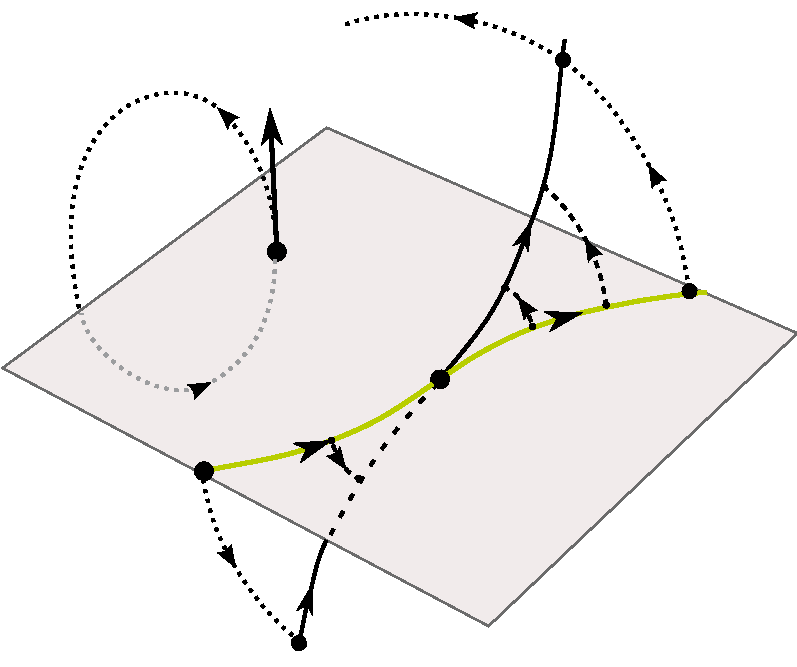
\includegraphics[width=\unitlength]{ReducTraj5.pdf}}%
    \put(0.09054399,0.38282057){\color[rgb]{0,0,0}\rotatebox{-30.34758661}{\makebox(0,0)[lb]{\smash{$\pSRed$}}}}%
    \put(0.57768586,0.29773425){\color[rgb]{0,0,0}\rotatebox{0.0313674}{\makebox(0,0)[lb]{\smash{$\sspRed(0)$}}}}%
    \put(0.59310014,0.69932675){\color[rgb]{0,0,0}\rotatebox{0.03136739}{\makebox(0,0)[lb]{\smash{$\ssp(\tau)$}}}}%
    \put(0.8268425,0.39772328){\color[rgb]{0,0,0}\rotatebox{0.03136739}{\makebox(0,0)[lb]{\smash{$\sspRed(\tau)$}}}}%
    \put(0.81220962,0.66529577){\color[rgb]{0,0,0}\rotatebox{0.03136739}{\makebox(0,0)[lb]{\smash{$\LieEl(\tau)$}}}}%
    \put(0.23150193,0.63610779){\color[rgb]{0,0,0}\rotatebox{0.0313674}{\makebox(0,0)[lb]{\smash{$\LieEl\,\slicep$}}}}%
    \put(0.37740434,0.49597258){\color[rgb]{0,0,0}\rotatebox{0.0313674}{\makebox(0,0)[lb]{\smash{$\slicep$}}}}%
    \put(0.3627714,0.69665188){\color[rgb]{0,0,0}\rotatebox{0.0313674}{\makebox(0,0)[lb]{\smash{$\sliceTan{}$}}}}%
  \end{picture}%
 \end{center}
 \caption{\label{fig:ReducTraj}
 % (b)
\Slice\ \pSRed\ is a hyperplane \refeq{PCsectQ}
passing through the {\template} point $\slicep$,
and normal to the group tangent $\sliceTan{}$ at $\slicep$.
It intersects all
group orbits (indicated by dotted lines here) in an open
neighborhood of $\slicep$.  The full
\statesp\ trajectory $\ssp(\tau)$ and the \reducedsp\
trajectory $\sspRed(\tau)$ belong to the same group orbit
$\pS_{\ssp(\tau)}$ and are equivalent up to a group rotation
$\LieEl(\gSpace)$, defined in  \refeq{sspOrbit}
(from \wwwcb{}).
 }%
 \end{figure}
													\toCB
Ponder whether to use \reffig{fig:ReducTraj} (current, but not updated
yet), or Fig~{fig:slice} in ChaosBook.org
How it was drawn is described in
\\
dasbuch/book/FigSrc/inkscape/00ReadMe.txt

  \item[2010-12-06 PC]
% ES 2010-01-19  Rescued from FrCv11.tex flotsam:
{\bf Tessellation of the \reducedsp\ by two or many slices:
how to implement it?}
Our proposal is essentially to approximately
\HREF{http://en.wikipedia.org/wiki/Voronoi_tessellation} {Voronoi
tessellate} (see \HREF{http://en.wikipedia.org/wiki/Voronoi_diagram}
{wiki on Voronoi diagrams})
We have to study Roweis  and Saul\rf{RoSa00}
\emph{``Nonlinear dimensionality reduction by locally linear embedding.''}
A sobering fact: Roweis, assistant professor at N.Y.U., a young
star in the field and universally liked, jumped out of his Washington
Square apartment earlier this year.

 This tessellation is akin to the
%\HREF{http://en.wikipedia.org/wiki/Vector_quantization}
{`vector quantization,'} (`block quantization,'  `pattern matching quantization'),
a computer science data compression method where sets of points are
clustered by their distance to `prototype' or `reference' points.
In computer science and linear programming a related method
is called \HREF{http://en.wikipedia.org/wiki/Vector_quantization}{`vector
quantization,'}
    \PC{credit Sara A. Solla with this observation}
(`block quantization,' `pattern matching
quantization'), a lossy data compression method where sets of points are
clustered by their distance to `prototype' or `centroid' points.
The
method is `lossy,' as in the replacement of a point by its `prototype,'
one drops the residual, \ie, the Euclidean distance between the two. It
works by encoding values from a multidimensional vector space into a `a
codebook,' a finite set of values from a discrete subspace of lower
dimension; \ie, what in the theory of dynamical systems is called
`symbolic dynamics.' Only the index of the codeword in the codebook is sent, thus
conserving memory and increasing compression. Vector quantization
numerical algorithms are unlikely to be useful to us.

% in part clipped from
% www.cs.unm.edu/~terran/downloads/classes/cs529-s10/docs/pretest_soln.pdf
An (affine) hyperplane is the locus of points obeying the equation:
\[
\sliceTan{1}\sspRed_1 + \sliceTan{2}\sspRed_2 + \cdots + \sliceTan{d}\sspRed_d = c
\,.
\]
In vector notation $\braket{\sspRed}{\sliceTan{}{}^{(j)}}=0$. In the case
of a slice the extremal distance condition sets $c=0$, so all our slices
include the point at the origin, $\sspRed=0$, and are not affine. A
$(d\!-\!1)$-dimensional hyperplane embedded in a $d$-dimensional space
and passing through the origin is defined by a normal vector \sliceTan{},
a vector orthogonal to every vector in the hyperplane (\sliceTan{} is the
primary object, the {\template} \slicep\ secondary in this way of thinking).
The intersection of two hyperplanes is a $(d\!-\!2)$-dimensional
hyperplane - the `ridge, `boundary,' or `edge' where two hyperplanes
meet. The intersection is $(d\!-\!2)$-dimensional because every vector in
the intersection must be orthogonal to the normals of both hyperplanes.
It is a $(d\!-\!2)$-dimensional hyperplane which also goes through the
origin. If you are an ant crawling along the trajectory $\sspRed(\tau)$
symmetry-reduced with respect to the first slice, you do not need to
compute this hyperplane. Every so often you compute
$\braket{\sspRed(\tau)}{\sliceTan{}{}^{(2)}}$. As long as this number is
negative, you have not gone too far. The moment it changes sign, you the
ant have crossed ridge, we symmetry-reduce with respect to the second
slice, and the ant continues its merry stroll along the second slice. We
do not need to be very precise about the instant where we switch, as long
as we are far away form wither slice's singularity subspace, so the ridge
can be `fuzzy,' and the numerical check infrequent and cheap.

There is a rub, though - you have to figure out how to pick the phases of
different \template s $\sliceTan{}{}^{(j)}$ in such way that you somehow
minimize the distance from one to the next as you cross the ridge. We
proposed in \refref{SCD07} to use heteroclinic connections for that - they
fix the relative phases of different \eqva.


 \item[2010-01-19 ES: Roweis and Saul\rf{RoSa00}] is indeed a very interesting
  paper that got me thinking again -- so much that I took the day off to devote
  it to symmetry reduction.

  The main goal is to construct a global, low dimensional ``intrinsic''
  embedding of high-dimensional data based on locally linear transformations.
  I will mention the three steps involved very briefly (but they will only make
  sense once one reads \rf{RoSa00} or the more detailed \rf{SaRo02}):
  (1) compute for each state space point its
  closest neighbors (within the sampled data), (2) solve a costrained
  least squares minimization problem for the (local) linear transformation
  matrix $W_{ij}$ that most accurately reconstructs each data point
  from its neighbors. (3) Given $W_{ij}$ (only!) solve a second minimization
  problem for the coordinates of each data point in a new, lower-dimensional,
  global coordinate system. In practice this involves solving a sparse
  eigenproblem for the first $d$ eigenvectors, where $d$ the dimension of
  the embedding.

  Roweis and Saul argue that the transformations computed in step (2) are
  translation, rotation and scaling invariant by construction and certain
  constraints imposed. This would fit us very well, but do we really want
  to also compute a low dimensional embedding? In principle this is what we are
  after, but we also do not want to make any drastic approximation of the
  dynamics at this stage.

  One option might be to reduce only by the group dimension.
  However one has to consider at least as many closest neighbors
  in step (1) as the dimension of the embedding. Then I would think that
  the problem might be computationally very intensive.

  Another option would be to bypass step (2) altogether and use a local
  moving frame transformation to map the local neighborhood of (a few?)
  sample points to local slices, then use step (3) to construct a global
  coordinate frame.

  In any case we might need to work with a symmetry invariant norm for the
  minimization problems, rather than the Euclidean distance used in \rf{RoSa00}.

  I would be very interested to try something else in a system without symmetry
  (e.g. KSe in antisymmetric subspace). Take the sample points from a dense
  set of periodic orbits. Rather than computing the  local transformation
  $W_{ij}$ in step (2), use the Jacobian of the periodic orbits
  (or use something Lyapunov vector related, if we get into this).
  Compute the global embedding as in step (3). Does it faithfully reproduce
  the dynamics? Can we learn something about the dimensionality of
  the attractor (actually of the embedding manifold)?

  There are $\sim1500$ papers citing \rf{RoSa00} so it is impossible to track
  all of them down. The ones from physics and math are fewer and the only one
  directly relevant to us I could find is by Bollt\rf{bollt07}.
  It does however use a different pattern recognition method (called ISOMAP)
  to compute embeddings of various systems, including KSe in antisymmetric
  subspace (no continuous symmetry reduction there).

\item[2011-01-24 PC] I know about ISOMAP and have decided that for us
it is a bad idea. Will blog that some other time.

\item[2011-02-04 ES] But what do you think about this method of Roweis and
Saul? It seems to do much better than ISOMAP for pattern recognition.
The important point that distinguishes it from ISOMAP appears to be that
it respects spatial relationships between neighboring points and
also conserves lengths.

\item[2011-01-24 PC] Made a claim in the slice \&\ dice article:
``
What about the fixed-point subspace $\pS_\Group$?
Because of it, the action of \Group\ is globally neither free nor proper,
\etc. All intersections of slices, ridges and {\sset s} contain the
fixed-point subspace $\pS_\Group$. Should we worry? Not really. The
objective of the \mslices\ is to freeze all equivariant coordinates; once
frozen, they together with the  $\pS_\Group$ coordinates span the
symmetry-\reducedsp.
''

Hope that is right. Have a further claim - it's easy to perturb away from
the fixed-point subspace $\pS_\Group$; in linear order the perturbations
commute, so equivariance implies the full reducibility of these
perturbations into block-diagonal components for each representations.
This is how it all started, with Ruelle\rf{ruell73}, but I think it is true
for \emph{all} perturbations from  $\pS_\Group$, not just the stability
of \eqva.

\item[2011-07-08 Predrag]
The $L^2$ norm of $\groupTan(u)$ is weighted by
the quadratic Casimir \refeq{QuadCasimir}. For \SOn{2} this is
$C_2^{(m)} = m^2$,
\beq
\oint \frac{d\gSpace}{2\pi}
     \, (\Lg u(\gSpace))^T \Lg u(2\pi-\gSpace)
= \sum_{m=1}^\infty m^2 \left(a_m^2 + b_m^2\right)
\,.
\ee{tangL2norm1}




\item[2011-07-08 Predrag]
Ridges are of Lebesgue measure zero, no way you would hit them.

We do not need to be very precise about the instant
where we switch, as long as we are away from either slice's singularity
subspace.


\item[2011-07-08 Predrag, from \refref{FrCv11}]                     \toCB
At this point it is worth noting that imposing the global and fixed slice
%\refeq{PCsectQ}
is not the only way to separate equivariant dynamics into `group
dynamics' and `shape' dynamics\rf{BeTh04}. In modern mechanics and even
field theory (where elimination of group-directions is called
`gauge-fixing') it is natural to separate the flow {\em locally} into
group dynamics and a transverse, `horizontal'
flow\rf{Smale70I,AbrMars78}, by the `method of
connections'\rf{rowley_reduction_2003}. From our point of view, such
approaches are not useful, as they do not reduce the dynamics to a
lower-dimensional \reducedsp\ $\pS/\Group$.

\item[2010-09-28 ES: Faddeev-Popov ghosts]                    \toCB
(moved to here from froehlich/blog)
\\
From my random readings, supposedly making up for my inability to attend
colloquia in French: Faddeev in a
\HREF{http://www.scholarpedia.org/article/Faddeev-Popov_ghosts}{scholarpedia
article} discusses the difficulties in Yang-Mills quantization that led
him and Popov to introduce fictitious fields, now known as
\emph{Faddeev-Popov ghosts}. The problem was that of gauge fixing,
essentially of working on a slice. Faddeev says:

\begin{ttfamily}
It was clear that the equivalence principle had to be taken into account.
In the functional integral framework, the equivalence principle implies
that one has to integrate over classes of gauge equivalent fields instead
of integrating over all fields $A_\mu^a$.

The choice of the representatives in the classes of equivalent fields is
realized by means of a gauge condition (gauge fixing), for instance,
\[
    \partial_{\mu} A_{\mu}^{a} = 0 .
\]
This condition defines a plane in the set of all fields, which is
intersected by the gauge orbits defined by
\[
    A_{\mu} = A_{\mu}^{a}t_{a} \to A_{\mu}^{\Omega}
            = \Omega A_{\mu} \Omega^{-1} + \partial_{\mu} \Omega \Omega^{-1} .
\]
In this context, the difference among abelian and non-abelian cases
becomes clear. In the abelian case, we take $\Omega(x) =
\exp{i\Lambda(x)}$ and a gauge orbit is defined by
\[
    A_{\mu} \to A_{\mu} + \partial_{\mu} \Lambda ,
\]
which is just a linear shift. Thus all the abelian orbits intersect the
gauge surface at the same angle.

In the non-abelian case, the gauge orbit equations are non-linear and the
intersection angle depends on the field parameterizing the orbit. It is
clear that this must be taken into account in the functional integral.
\end{ttfamily}

See the wikipedia link to put this in the proper context. As an abelian
case Faddeev lists quantum electrodynamics where the group is $U(1)$ (the
same as in \cLe\ if we think in terms of complex variables). As a
non-abelian example he lists the Standard Model: $U(1)\times SU(2) \times
SU(3)$.

Faddeev relies on the group being connected to write group action in
exponential form, as Stefan does. $\On{2}$ in Kuramoto-Sivashinsky is
non-abelian so I am worried that there might be more work required. Are
all non-connected compact Lie groups non-abelian and vice versa?

The weight factor Faddeev and Popov introduced might be helpful in
trace-formulas for non-abelian groups.

\item[2011-12-06 Roman] However,  ECS can be used to project
trajectories onto a low-dimensional visualization where coordinates $a^k_{i}(t)$
are defined by the inner product
\beq
\label{coordinatesRG}
a^k_{i}(t)= \frac{1}{V} \int_V {\bf e}^k_i(t)^\dagger\cdot({\bf u}(t)-{\bf u}^k(t)) dV,
\eeq
%\pagebreak
where $V$ is the flow domain volume, ${\bf u}^k(t)$ is the ECS closest to
the system state at time $t$, and ${\bf e}^k_i(t)$ are basis functions
representing a set of unstable and weakly stable modes characterizing the
particular ECS.

\item[2011-12-06 Predrag]
Mhm - why are we introducing new notation for \statesp\
coordinates in \refeq{coordinatesRG}? I cannot imagine a situation in which one
would like to make the bases  ${\bf e}^k_i$ time dependent, ${\bf e}^k_i(t)$,
and we mostly use ECS themselves to construct projections, as in
\reffig{f:ssptransient}, not their stability eigenvectors. If you are really
thinking of using ECS's ${\bf u}^k(t)$ as \template s whose linearized local
charts compose a global atlas for the flow, they would not be time dependent,
but fixed by a set of Poincar\'e sections to \statesp\ points ${\bf u}^k$, and
the associated set of unstable and weakly stable eigenvectors (what are
"modes"?) ${\bf e}_i^k$ would also be confined to the Poincar\'e section, and
not time dependent. But I think this is way too sophisticated for referees to
wrap their heads around....

I propose you drop time dependence from ${\bf e}^k_i(t)$ and ${\bf
u}^k(t)$ and pass over all that in silence for now. Or perhaps keep the
formula as is, as neither the authors themselves have never sorted out
how the \po\ eigenvectors are to be used in practice.

\begin{figure}
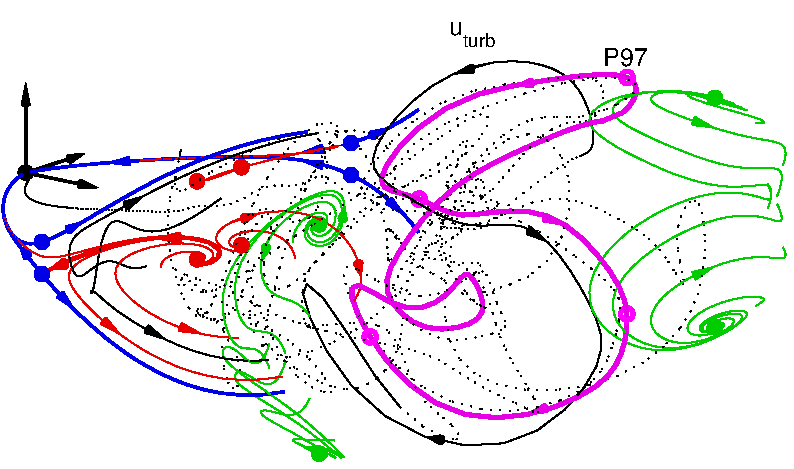
\includegraphics[width=0.4\textwidth]{P97portrait5}
\caption{
{\bf A state-space portrait of turbulent plane Couette flow.}
A turbulent trajectory ${\bf u}_{\text{turb}}$ (solid and dotted black
lines) shadowing the P97 periodic orbit (bold magenta line) and the
unstable manifolds (blue, red, and green lines) of symmetry-related
equilibria (solid blue, red, and green dots; the black dot at the origin
is the laminar flow state). Velocity fields corresponding to the open
magenta dots on P97 are shown in  reffig~{f:ssptransient2}. Dynamic
connections are shown as bold red and blue lines connecting different
equilibria (filled dots).
}
\label{f:ssptransient}
\end{figure}

\item[2011-12-06 John] Predrag's comment on \refeq{coordinatesRG} is on
target: it makes sense with the verbal description attached to it, but
the time-dependence of the basis set $e_i^k(t)$ and the nearest ECS
$u^k(t)$ is pretty confusing. The bigger problem is that the equation as
is reflects what we want to do, but doesn't the projection in
\reffig{f:ssptransient}, which uses a fixed basis based on four
symmetry-related ECS to produce a global portrait.


\medskip


\item[2011-10-28 PC~~] to Ashley: Once you have a \rpo\ reduced to a
slice, as in \reffig{f:MeanVelocityFrame} or \reffig{fig:M1OrbMarc}, you
simply take any point $\ssp \in \RPO{p}$, and trace its group orbit until
next time it crosses the slice; then you trace out the image of the
$\RPO{p}$ that you already have. That produces no less than the two slices of
the \rpo, as in your own \reffig{fig:sliceimage}, but in general more, as is
illustrated by the Siminos \reffig{ks22rpo16mf}.

In any case, keep going on the same group orbit of a point of the one and
only good \po\ and check whether there are further crossings of the
slice; each will correspond to yet another bad \po. Please check the sign
of the curvature for each traversal of the slice. If you
start from the good, nearest \po\ and track the curvature as you move on
the group orbit, you will go through zero curvature - such points mark
crossing the {\sset} $S$, \ie\ the border of the slice. It is verbotten
to cross on the other side - there you are outside our atlas of the
world.

\item[2011-10-28 PC~~] to Ashley:
    define the bulk velocity $U$ in the text, refer to it in
    \reffig{f:MeanVelocityFrame}\,{(a)}. Isn't it sufficient to just plot
    $\vec{u}$, the deviation \refeq{NavStokesDev}? APW: It moves so
    rapidly that the plot would be an unfair comparison -- points
    sufficiently close to make smooth curves here plot as random points
    otherwise.  {\bf PC:}  I guess I do not understand. $\vec{u}(\zeit)$
    for $\RPO{36.92}$ traverses many $L$ streamwise lengths in period
    $\period{}=36.92$? Can you define $U$ in the text, refer to it by the
    equation number in the caption.
    {\bf APW} It traverses approx 8 times!  $U$ is the same $U$ used
    in the definition of the Reynolds number, hopefully clearer from
    slight rewording.

\item[2011-10-28 PC~~]: On using $\slicep$ as one of the coordinates: The
state vector $\ssp$ is not normal to \normVec(\ssp), as $\braket{\ssp
\Lg^2}{\ssp} = - \Norm{\groupTan(\ssp)}^2 \neq 0$, but can one use it to
produce from $\ssp$ the 3. local eigenbasis unit vector? Have not thought
that through. If we do that here, need to rewrite text leading to
\refeq{PCsectQ0}.

\item[11-11-04 APW~~] Why is curvature mentioned in the caption of
\reffig{fig:sliceimage}? {\bf PC:} As you look at the closest point on a
group orbit, distance increases in all moves away from it along the group
orbit, \ie, the matrix of 2nd derivatives of the distance function has
only positive eigenvalues. For any local extremum that is not a local
minimum, there are negative eigenvalues, \ie\ directions in which the
distance decreases.

\item[2011-10-28 PC~~] to Ashley:
The rev.~127 version of the text: ``
The variational distance condition \refeq{PCsectQ0} is
only an extremum condition, and as the group orbits of highly nonlinear
states are highly contorted (see see \reffig{fig:2830GO6}\,{\it b}), they can
have many extrema, and multiple sections by a \slice\ hyperplane. For
example, a single \rpo\ is typically intersected by a \slice\ hyperplane
in several separate sections of the \rpo\ torus, see
\reffig{ks22rpo16mf}.
''


\item[2011-10-20 APW~~]
\refFig{ks22rpo16mf} remains in the body tex,
which is what I was asking to be moved previously, and I'd prefer to omit
-- I think it'd be a real bugger to produce for the pipe orbits!
{\bf Predrag 111020} please give it a try for the $\RPO{36.92}$ - maybe
not so bad; hopefully not too many charts needed, especially if you use
as {\template} a point on $\RPO{36.92}$.
[see above: Ashley did replace it by \reffig{fig:sliceimage}]


\item[2011-10-28 PC~~] Marc, I've been pondering how to explain the
difference between using physical states to triangulate high-dimensional
\statesp s, and projections on a few primitive integration variables.
Maybe this helps (not suitable for this paper, but maybe you and Ashley
can see a way to communicate that fails me).

I will add this text to \refappe{appe:slice}, also including
    ``The problem we are facing is this: the inertial manifold
(or, more precisely for a dynamicist, the nonwandering set) is a
finite dimensional, presumably highly contorted nonlinear manifold
\citep{foias88}
embedded in our particular representation $\infty$\dmn\ vector \statesp.
Our strategy is: (1) shift the origin to a point embedded in the
inertial manifold. (2) construct an efficient atlas of the inertial manifold
by selecting a minimal set of \template s embedded in it, with associated
local hyperplanes that reduce the continuous symmetries (slices) and the
continuous time (Poincar\'e sections).
''

    ``More straightforward visualizations are based on choices of several Fourier
components \refeq{pipeDiscr} or other primitive basis elements as
coordinate axes for projections of the flow. They are appropriate for
small perturbations off laminar state, but such coordinate axes are (i)
arbitrary and discretization-method dependent, and (ii) point in
unphysical directions, far from turbulent states which in a highly
nonlinear flows are characterized by  many strongly coupled Fourier modes
of comparable magnitude.''

``The {\stateDsp} portraits are {dynamically intrinsic}, since the
projections are defined in terms of intrinsic solutions of the equations
of motion, and {representation independent}, as the inner product
\refeq{innerproduct} is independent of the numerical discretization.
''



\item[2011-10-25 John Gibson~~]  to Predrag: ``         \toCB
Chart or atlas is fine by me. We'll have some more 'splainin' to do for
the poor dumb plumbers. I think ``chart'' refers to be the set of
local maps from the manifold to a Euclidean space, and we will only ever
be dealing with maps between Euclidean spaces.
'' Here is what we wrote in a recent proposal: ``
{\em Patchwork dynamical models}. [...]
The long-terms goals of our research program are to develop this vision into
quantitative, predictive description of moderate-{\Reynolds} turbulence, and
to use this description to control flows and explain their statistics. The
first step, and the main subject of our theory proposal, is to build an explicit
instance of such a model for PCF in a minimal flow unit. A large set of
unstable periodic orbits for this flow have already been calculated\rf{CviGib10}.
We will compute the unstable eigenmodes of these orbits, continue their
unstable manifolds by time-integration of small perturbations, and thus map
out the conditions under which one unstable state transitions into another.
We will build a catalog of allowed transitions between ECS and calculate
the linearized dynamics in the low-dimensional unstable manifold about each
unstable periodic orbit. This will form a ``patchwork'' model of the turbulent
dynamics: an arbitrary fluid state will modeled by a low-dimensional
linearization in the unstable manifold of the nearest ECS, with the model
jumping from linearization about one ECS to another.
''


\item[2011-10-25 MA~~] back. Will work for food. I believe I understand
why Gibsonian coordinates are useful and accept their superiority; they
are well suited to look at phase space locally, while Fourier modes only
locally to the laminar state (i.e. useless in pipe flow). But many
people, including Mellibovsky \& Eckhardt (2011) and the sequel in the
arXiv do this. My suggestion was just to make a Fourier plot to compare
it to Gibsonian and be pedagogical...
\\
{\bf 2011-10-25 Predrag} Using Fourier modes is like standing in the
lower left corner of a soccer stadium, and trying to kick the ball which
is by the opposite goal. Best to try it yourself. You'll be enlightened
if you plot the $\RPO{36.92}$ as
$(\vec{u}_{327},\vec{u}_{253},\vec{u}_{199})$, compare with Ashley's
masterly physical projections. As to Eckhardt - I did the stupid thing
myself from 1996 to 2005 \refref{Christiansen97} until impossible, and we
realized that elementary ideas about vector spaces work better
\refref{GHCW07}.
\\
{\bf 2011-10-25 Predrag} the surprising thing about `physical' coordinates
(any better name to call them?)
is that they are so good \emph{globally}, that is what all plots in
\HREF{http://ChaosBook.org/tutorials}{ChaosBook.org/tutorials} are.


\item[2011-10-28 PC~~]
This has come to pass: China is getting modern at a frightening pace, I
have a \emph{lazy } Chinese student. He finally showed me on the screen
his undocumented Matlab plots of \KS\ \rpo s in co-moving frames. He does
not use any variant of my $\{\be_a, \be_s, \be_m\}$ orthonormal
`physical' basis \refeq{intrSspTraj} in spite of my many attempts to
explain it, and I suspects he does not understand what it is, until there
are plots that show the contrary.

\medskip

He plots \rpo s in `real space', meaning 3 components,
\[
\mbox{let's say } \{x_{47}, x_{48}, x_{49}\}
\,,
\]
of the 64-dimensional \KS\ discretization
vector that the integrator returns, with the mean {\phaseVel} per period
subtracted. \Rpo s do close into \po s. The shortest one looks like a
nice circle, longer ones are not a pretty sight. He has no clue that
there is FFT hidden in the integrator (or presumably what FFT is), so he
cannot plot your Fourier modes, but I think you see what the problem is
more clearly this way.

\medskip

It is as if Bjorn chose to look at 3 pixels of a
video image of one of his turbulent flows, and from that proceeded to
reconstruct the full turbulence. It cannot be done, even in principle;
it's like using a hot wire in a wind tunnel in 2011. What I offer to
Bjorn instead is a full resolution $3D$ snapshot of a turbulent state
(that is also a point in \statesp, but now the basis vector goes straight
through  it, and all pixels are retained), and ask him to compare his
measurement (a nearby point in \statesp) to my snapshot. That is a powerful
theory.

\medskip

Looking at a known \rpo\ is a bit misleading in this context. A circle
will close into a circle in any projection, as long the turbulent state
is global, as its \statesp\ trajectory generically has projection on all
of the $\infty$-many axes, but it is still a series of 3 pixels video.
You cannot work out the catalogue of turbulent states this way.

\medskip

Am I reaching you? If yes, can you put it in words that your colleagues
will understand? It is not about accepting superiority of Gibsonian
coordinates, it is about how to discuss this with fluid dynamicists. Even
Gibson does not understand this - since then he has fallen back to his
fluid-dynamicst's roots, it's all about bifurcations, snaking and plotting
things in the parameter-energy plane.


\medskip

The whole process of communal learning and myths fascinates me. Often one
encounters group mental states where all agree on something that is
patently a nonsense. Not just string `theory', or climate change deniers.
Plumbers' `energy' has no meaning other than that numerical people can
plot it because their codes happen to spew out Eulerian velocities. Ask
Bjorn to measure it... People click on a wiki, they exchange a nod of
agreement with a colleague and collectively psych themselves into
believing that they have understood. There are too many things, one
cannot learn them all, so groups work by consensus. It must have been
different 100 years ago when there were handful people interacting -
otherwise we still would not be using Cauchy's contour integrals and
quantum mechanics - those were inventions that really required exercising
neurons. Here we are picking axes in a linear vector space.

\medskip

But I digress...


\item[2012-02-21 PC]  I like the way this chaos class is working, and I
think we can put together some of the best class contributions into a
pedagogical article about sections and slices. And we have a chance to
publish this in a high quality issue of one of the better journals in the
field, Chaos:

\item[2012-02-21 Phil Holmes to PC]
We write in connection with the recent IUTAM Symposium on 50 Years of
Chaos: Applied and Theoretical, held in Kyoto, which you attended. In
addition to the Conference Proceedings to be published by Elsevier as
part of their regular IUTAM series, the American Institute of Physics
(AIP) has agreed to devote a special issue of the AIP Journal
\emph{Chaos} to papers representing a selection of the topics presented.
This is planned to appear as \emph{Vol 22 (4), December 2012}. So far 11
invitees have agreed to contribute papers; only one (David Ruelle) has
declined.


Based on your interesting presentation in Kyoto, we would like to invite
you to submit a paper for consideration for this special issue of Chaos.
Please let us know as soon as possible if you would like to do so, at the
latest, before Monday Jan 16th, 2012. Papers may either review a topic,
preferably including new results, or present entirely new, unpublished
results; papers should also reflect the topics and themes presented at
the symposium. All contributions will be refereed in the usual manner, as
for unsolicited submissions to AIP journals. At present we expect this to
require submission of the paper by \textbf{March 30th, 2012}, with
resubmission of revised papers during June 2012.


\textbf{[NOTE from Phil Holmes]}
Since some of the work you described has appeared in previous papers, in
particular that on channel flows with John Gibson, I would be especially
interested in the new results on symmetry groups hinted at in your
presentation.


\item[2012-02-21 PC to Phil Holmes]
Thank you for your kind invitation to contribute to the special issue of
the AIP Journal Chaos in connection with our "50 Years of Chaos". I am
sorry I am responding past your deadline, but I was not sure we would
have results interesting enough to report in this issue, results that
have not been written up for other publications. Now I am feeling more
confident that we can offer a novel pedagogical review of the symmetry
reduction by the method of slices (that I had described by its
application to one example, the pipe flows, in Kyoto), so I would like to
join this very fine group of contributors to the planned December 2012
Chaos.

\item[2012-02-23 PC] For instructions read
\texttt{siminos/atlas/Chaos-v1/00ReadMe.txt}. The deadline is

\textbf{April 16, 2012}

\item[2012-01-27 Predrag]
    please, as few \template s as possible in \reffig{fig:thetadot2}.
    (and do not keep renaming this figure :-) And there should be no
    jumps in $\dot{\gSpace}(\sspRSing)$, none at all. We just need to
    make sure that the ridges between the \template s are sufficiently
    close to each the \template s, so that the {\sset s} are excluded. Once
    \template s are picked, the rest is geometry of hyperplanes (NOTHING to
    do with dynamics, only with the group theory) so checking whether the
    {\chartBord} is on the far side of the tile edge (ridge
    between two \slice s) is a linear computation, to be undertaken
    independently of dynamics.

    If the jumps are genuine and non-removable by refinements of slice
    charts, that's a big deal. It indicates that the generic turbulent orbit
    makes arbitrarily close passages to invariant subspace(s), and that is
    physical, not a chart artifact. Are there physical states that are like
    Hagen \eqv, but stream-wise deformed, \ie\ is there a nontrivial subspace
    invariant under the whole symmetry $\Group = \On{2}_\theta \times
    \SOn{2}_z$?

\item[2012-02-18 Predrag] clippings

This procedure has been devised by Poincar\'e in the context of celestial
mechanics, in the aim of reducing the analysis of long-term planetary
motion and its dynamic stability [Poincar\'e, Les m\'ethodes nouvelles de
la m\'ecanique c\'eleste 1892].

\begin{figure}
  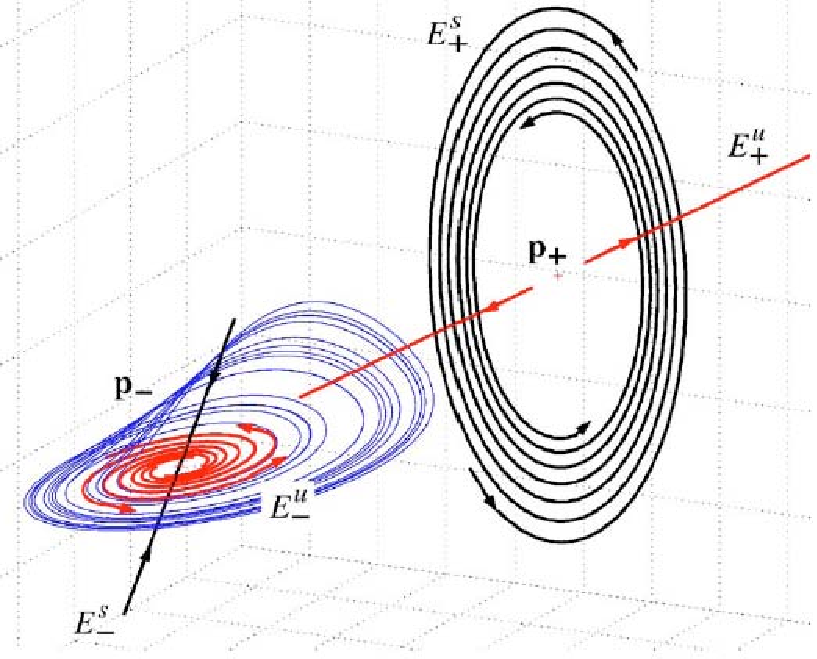
\includegraphics[width=0.4\textwidth]{AmLeAg06Im1}\\
  \caption{From \refref{AmLeAg06}:
R\"ossler attractor with fixed points and their manifolds. The linear
stable manifold at the lower fixed point is 1-dimensional and the
unstable one is associated with an unstable focus. The stable manifold at
upper fixed point is a stable focus and the unstable manifold is
1-dimensional}
\label{fig:AmLeAg06Im1}
\end{figure}

From \refref{AmLeAg06}:
``A linear system is $\dot{x} =Ax$ and an affine system is $\dot{x}
=Ax+b$, where $A$ is a constant matrix and $b$ is a constant vector.''

                                            \toCB
Draw (un)stable eigenvectors as in \reffig{fig:AmLeAg06Im1}. Also, run
the unstable spiral(s) for the upper brunch further out, to trace out the
basin boundary.


``
In the R\"ossler system, the switching is induced by the nonlinearity
which acts when the trajectory is sufficiently far from lower fixed
point, that is, beyond the threshold $x-c$ in the third equation. The
nonlinearity acts when the trajectory is sufficiently close to upper
fixed points where its converging spiral induces the folding by sending
the trajectory back to the neighborhood of lower fixed point along its
unstable manifold. Thus, the lower fixed point is mainly responsible for
the stretching and upper fixed point for the folding.
''

\item[2012-03-02 Predrag] Francesco likes my explanation why Euclidean
invariance leads to spirals. Imagine a thousands of marines parachuted
into Sahara desert an overcast night with no wind. Turn off their GPSes,
and order each one of them to march straight to Tripoli. The chance that
anyone will walk a straight line is zero - at best they will circle, or
spiral away from where they started. In presence of symmetry, and no cost
for moving along the group manifold, and no possibility to flip the
direction of motion, all motions will be drifting.

\item[2012-03-02 Predrag]
A Modest Proposal: create along with this article a Slice \& Dice
tutorial, like the \HREF{http://chaosbook.org/tutorials/index.html}{\pCf
one}. I believe Mathematica has ability to put user-orientable 3D
graphics into a browser, or HTML5 has that facility - that would make
slicing much easier to understand.

\item[2012-02-28 Predrag]
    The big problem with \reffig{fig:thetadot2} \template s
    is that they belong to the set of \reqva\ that has nothing to do with
    turbulence. It would be better to use points from $\RPO{36.72}$ and
    some \template s picked from most likely the turbulent trajectory
    states.

    The problem with \reffig{fig:thetadot2} that you never explain how
    you chose \emph{relative phases} between \template s. I think the way
    it should be done is that in the starting slice\ $\pS{}^{(1)}$, a
    local chart at $\slicep{}^{(1)}$, you plot both points corresponding
    to group orbits of other \template s, and keep checking the distance of
    $\sspRed(\zeit)$ to all $\slicep{}^{(j)}$. The moment one of them,
    let's say $\slicep{}^{(2)}$ is closer to $\sspRed(\zeit)$, you keep
    that $\slicep{}^{(2)}$ (that fixes the relative phase) switch to its
    slice\ $\pS{}^{(2)}$, and keep checking distances there. You cannot
    just pick a random set of points, one on group orbit of each {\template}
    - slices so constructed can sit anywhere in the full \statesp. It is
    not a technicality - it is the reason why the shift (red line in
    \reffig{fig:thetadot2}) is still too kinky, and probably the reason
    why no good guesses for \rpo s embedded deeper in the turbulence have
    not emerged as yet.

\item[2012-03-09 Bryce Robbins]
After diligently working on properly charting the state space of the
complex Lorentz flow I have successfully produced an atlas whereby the
singularities have been removed from the reduced flow!

\item[2012-03-09 Bryce]
Now the only issue I am running into now is how to merge two successive
trajectories in a given chart. For example: I am currently using 2
charts, whenever the value of  $|\dot{\gSpace}|>1$  I rotate the final point
in the iteration into the other chart and start integrating in that
respective chart.

\item[2012-03-09 Predrag]
Do you really mean  $|\dot{\gSpace}|>1$? That seems far from $|\dot{\gSpace}|
\to \infty$, and $|\dot{\gSpace}|=1$ could be perfectly physical, especially
in some other slicing problem. How about checking the sign of chart
border condition,
\(
\langle{t(\hat{\sspRed}(\zeit))}\vphantom{ }|\vphantom{}t'\rangle= 0
\,.
\)
When this expression has changed sign, you have gone too far - backtrack
and change the chart.

\item[2012-03-09 Bryce]
Every time the code breaks I append a large array of data for each chart
with the new trajectory data. After all is said and done I have two
arrays each containing a bunch of data that is disconnected in certain
areas (namely the points where the integration ended and started back up
again when a new starting point was rotated into the chart from the other
chart). If I just iterate once I can join each dot in a 3D list plot,
however, in the final data set the jumps prevent me from connecting these
lines. If I do draw in the lines connecting the points I end up with
lines streaking across the symmetry reduced trajectory which is of course
very undesirable.

Any ideas to mitigate this?

\item[2012-03-09 Predrag]
As how to connect the two charts - have to think. I thought they connect
continuously on the ridge (intersection of the two \slice\ hyperplanes).
They do not?

The main thing (without which there might be no paper) is showing that
two templates suffice to slice SO(2) for complex Lorenz. Bryce has chosen
two points on the group orbit = time orbit of the relative equilibrium. I
believe that is wrong, because in any slice all points on a relative
equilibrium correspond to the unique equilibrium.

My feeling is that the other template should be as far as possible but
within the non-wandering set: Something close to the equilibrium at the
origin. Cannot be the equilibrium itself, as it is in the fixed-point
subspace, and there are no group tangents there.

I am not sure one can find two charts that do the job - as I have not
done it myself. But if it is impossible, the explanation why not might be
very interesting....

\item[2012-03-16 Bryce]
I'm going to try to resolve this issue of choosing two sufficient charts
for the complex Lorentz flow over the course of the next couple of days.
Based on what I have computed, I have a feeling that it is possible and
if not we might simply need more than two charts as you've suggested. I'm
going to plot the \chartBord\ in both charts I choose to see
if they are even sensible before I go about computing the dynamics. When
I make some significant headway I'll inform you of my progress. If you
have any ideas that pop into to your mind in the meantime let me know and
I'll try to implement them.

\item[2012-03-16 Predrag]
slice is 4-dimensional, so the chart border is 3 dimensional - do not
know how to visualize that in any 2- or 3- dimensional visualizations.

Only thing I can think of is to track $\dot{\theta}$ for $\hat{x}(t)$,
until it gets rather large, make sure it happened beyond the ridge to the
next chart.

\item[2012-03-09 Bryce]
As I am plotting the reduced state space trajectory in only three
dimensions (x1, x2, z) so I should be able to find the border on the
slice. I do not intend to visualize the four dimensional border in its
entirety but will project it onto 3 of the 5 dimensions. Will this be
sufficient enough to determine if the slice is a sensible slice?

\item[2012-03-16 Predrag]

%%%%%%%%%%%%%%%%%%%%%%%%%%%%%%%%%%%%%%%%%%%%%%%%%
% 2011-10-23 Predrag: ConicplaneSects.png
% from en.wikipedia.org/wiki/File:Conic_sections_with_plane.svg
% edited siminos/figSrc/inkscape/ConicplaneSects.svg
%
\begin{figure}\label{f:ConicplaneSects}
\centering
(a) %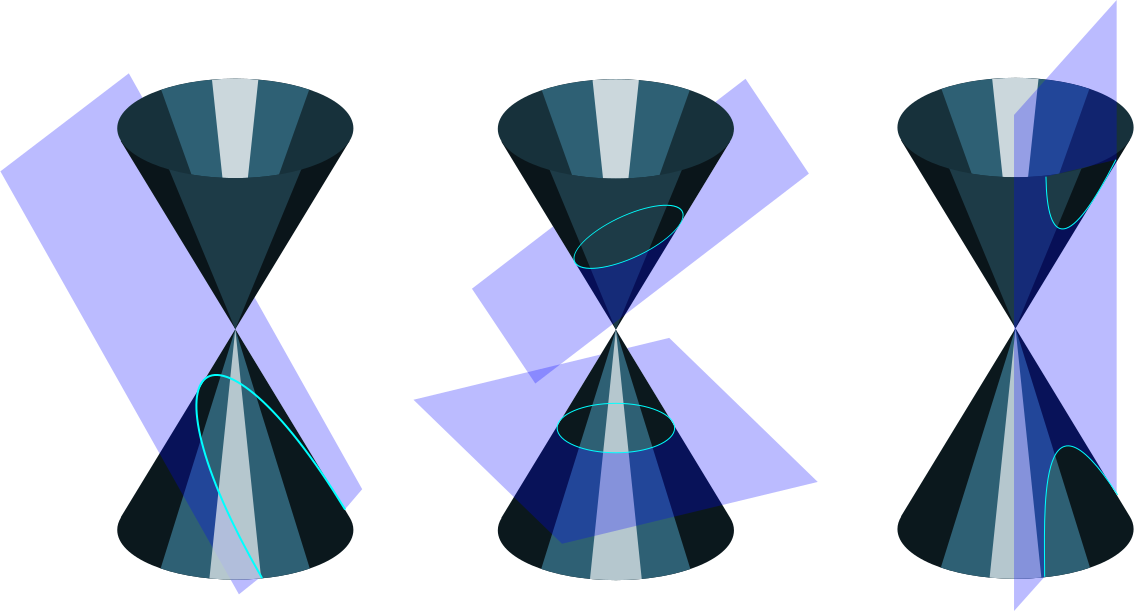
\includegraphics[width=0.45\textwidth,clip=true]{ConicplaneSects}
(b) %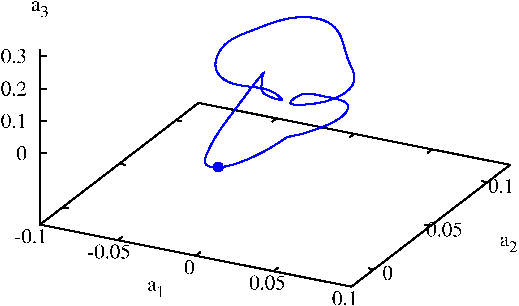
\includegraphics[width=0.45\textwidth,clip=true]{2841GO3b}
\caption{
(a) Conic sections (b)
}
\end{figure}
%%%%%%%%%%%%%%%%%%%%%%%%%%%%%%%%%%%%%%%%%%%%%%%%%%

\item[2012-03-11 Predrag]
Let's try to solve ChaosBook.org problem 3.2 (?) right, like any
high-school kid would do: look up
\HREF{http://en.wikipedia.org/wiki/Conic_sections}{Conic\_sections} in
Wikipedia, see \reffig{f:ConicplaneSects}.

\item[2012-03-10 Predrag to Daniel] I put soluChap10.pdf in Dropbox. In
the current edition the programs are renumbered. So far you have done:
\begin{itemize}
  \item[10.8]  An $\SOn{2}$-equivariant flow with two Fourier modes
  \item[10.10] $\SOn{2}$ equivariance of the 2-mode system
           for infinitesimal angles.
\end{itemize}
Next bunch of exercises to do:
\begin{itemize}
  \item[10.11] Visualizations of the 5-dimensional 2-mode system
  \item[10.22] 2-mode system in polar coordinates.
  \item[10.23] The relative equilibria of the 2-mode system
  \item[10.24] Plotting the relative equilibria of
           the 2-mode system in polar coordinates
  \item[10.25] Plotting the relative equilibria of
           the 2-mode system in Cartesian coordinates
\end{itemize}

Still have to make up exercises on group orbits, templates, slicing


\item[2012-03-18 Predrag]               \toCB
Use \reffig{fig:A27-pipeSymms} in ChaosBook.org. (to Predrag: remember to
copy them to dabook/book/Fig and FigSrc/). How it was drawn is described
in dasbuch/book/FigSrc/inkscape/00ReadMe.txt


% FIG. 11. A 2-chart atlas
\item[2012-02-25 Predrag to Chaos Gang]
It seems to take a workday to draw 3-4 figures, so the draft is still
problematic. But do please study \reffig{fig:A29-2slices}, it's a
concrete proposal how to slice the \cLf\ and the 2-mode model.

\item[2012-03-18 Predrag] I have added Siminos data (see {\bf [2010-07-12
ES]} above) to the Chaos Course Dropbox.com:
\\
          \texttt{SharedCode/CLErpos.dat}
            contains Evangelos Siminos data on four relative periodic
            orbits, symbolic codes 1, 01, 011, 001 you can use to test
            you code. The data is ordered as
            (T theta x1 x2 y1 y2 z Lambda1 ... Lambda4)
\\
          \texttt{SharedCode/CLEcycles4.dat}
            If you really want to go to town, a much larger set of
            relative periodic orbits, you can figure what is what by
            comparing with the 4-orbits data set above.

\item[2012-03-18 Predrag] My gut feeling is that a good 2. \template\ for
\cLf\ could be a point on the \cycle{01}-cycle; that is the short \rpo\
`furthest away' from the 1. \template\ \cycle{1}. \Eqv\ at the origin is
out, as it lies in the \Group-invariant subspace and has no non-zero
group tangents. \Template s should always be chosen fully equivariant,
otherwise they do not fix a slice.

\item[2012-03-20 Daniel]
Got the slices working for \cLf. Used the implementation from
ChaosBook.org ver. 13.7.3, sect. \emph{10.4.2 Dynamics within a slice},
rather than the post-processing method. Given a template my code can
slice away. I recreated figures 10.12 (attached) to check that it was
doing the right thing and they look pretty good.


\item[2012-03-20 Predrag  to Daniel]
You are still in the larval, single slice stage - if you look at your 2.
plot, (track magnitude of $\dot{\theta}$, \etc) you will find out that
you are going through singularity and jumping by $\Delta \theta = \pi$
every time you do it. All mindless integrators cheat their way through
this singularity, but if you want to see it in detail, have a look at
Figs. 3 and 4(a) in
\HREF{http://www.cns.gatech.edu/~predrag/papers/preprints.html\#FrCv11}
{www.cns.gatech.edu/$\sim$predrag/papers/preprints.html\#FrCv11} (and do
not ever publish figures so ugly - Stefan\rf{FrCv11} got waiver as an
undergrad and a mathematician).

\item[2012-03-20 Daniel]
What do you think would be the most productive next step? Modify the code
to slice the 2-mode system? Take slices of the complex Lorenz system with
templates that are not the equilibrium solution? Try to Poincar\'e
section the slices? Please advise. In the meantime, I'll clean up my code
so it makes sense to people when I post it.

\item[2012-03-20 Predrag  to Daniel] Let's get a 2-chart atlas working, then
we move to the next thing...

\item[2012-03-21 Daniel  to Predrag] Ok. Got the tunnel working so I can
read this stuff at home and actually take the time to blog. Couple of
comments:

Who is doing what? It seems like there is some duplication of effort in
this endeavor. One can sort of dig around the various blogs and such and
infer what people are working on, but it's kind of hard to tell. It seems
like at least Bryce and I are chasing the same result.

\item[2012-03-21 Predrag]
It's not duplication, for the students it's education. Ideally, everyone
in the calls should be able to do this (there are only two students who
are not seriously working), and anybody who contributes significantly to
the paper can be a co-author. The goals are very modest: explain
pedagogically the course lectures on symmetry reduction, in two steps:
(a) Carefully re-examine and illustrate on R\"ossler flow what is one
really does when one sections time trajectories: (b) Repeat the same on
slicing the the group orbits, illustrate by \cLf, both models with high
quality figures. I hope that by the students making sure the exposition
is pedagogical it will much more so than my papers have been.

In your case (and equally so for Radford and Chris, but they seem not to
have gotten the memo) I hope you will find this very helpful in your
research, so understanding is much more pressing than for the Chaos
Course.

I do not understand why it has been so difficult - I think that the
problem is that the senior people assume they have been knowing this, and
none of them do. I speak with some authority, as I know much more group
theory then 99\% of physicists, and I had not known these methods. Turns out
that nonlinear group theory is to linear, quantum mechanical methods what
linear ODEs are to nonlinear ones.

Spent two hours with Roman and Mike (sorry, should have thought of
calling you in to Roman's office, but I had assumed it would take only 15
minutes), and my chaos class understands this better than the pros. Maybe
it does.

\item[2012-03-21 Daniel]
It is also not totally clear to me where I should be saving code,
figures, blogging, etc., so that it is most useful to the group effort.
Predrag, please advise.

\item[2012-03-21 Predrag]
An attempt in \refsect{chap:outline}, edit as you see fit.

\item[2012-03-21 Daniel]
I had read the stuff in DasBuch about the singularities. I just wanted to
make sure that I was on the right track. Anyway, I guess the idea is to
jump to a different chart (hyperplane associated with a single template)
whenever you get close to the singularity (probably way before then, and
more like when you are closer to another template on another chart,
right?)

\item[2012-03-21 Predrag]
ChaosBook chapter is two years out of date - the current wisdom was only
given in my lectures and shuld be written up in the
siminos/atlas/atlas.tex paper. I will rewrite ChaosBook chapter after we
finish this paper and clock up a few more cutting edges research
breakthroughs. Please try to implement atlas construction as outlined in
\reffig{fig:A29-2slices}.

\item[2012-03-21 Daniel]
Is the 2-mode system still of interest or should we put that on the
back-burner and focus on the \cLe, even if the relative equilibria are
all circles? I've been writing two versions of every piece of code, one
for the complex Lorenz system and one for the 2-mode system (which is
still lacking a ``good'' set of parameters that make it nice and
chaotic). It's not too much work to make one once you have the other, but
there are details to be addressed, so work would go faster working on a
single problem.

\item[2012-03-21 Predrag]
Atlas for \cLe\ is the top priority. The 2-mode system is experimental,
maybe you can get a more interesting system from some truncation of the
2D Kolmogorov flow. That is totally open.

\item[2012-03-21 Daniel]
From some of the most recent comments copied from pipes/blog suggest that
Rich (I'm assuming Kerswell?) has been looking at periodic orbits in 2D
Kolmogorov flow. Perhaps, the third floor 2D crowd should be in touch
with these guys. Do Mike and Roman know about this?

\item[2012-03-21 Predrag]
Sorry, maybe it is my fault - I just assume everybody tracks the current
literature, I should have told them in person. Here is another relevant
blog entry:

{\bf 2011-05-18  Rich Kerswell} Read Irene Moroz, Geophys. Astrophy Fluid
Dynamics vol 105, 273-286, 2011, \emph{Unstable periodic orbits in 4D
Faraday disk dynamo}. Might give you a 4-dimensional dynamical system
which is chaotic and can be reduced to a 3\dmn\ \statesp; easier to
visualize than {\cLf}.

Kerswell papers are published and easy to find; if you learn something,
please summarize it here for the rest of us.

\item[2012-03-19 Predrag~~] Please study \reffig{fig:A29-2slices}, it's a
concrete proposal how to slice with several templates. Their relative
phases matter.

\item[2012-03-21 Marc~~] \refFig{fig:A29-2slices} is a very neat solution
to the problem of how to decide when to switch templates. Still, the
main problem I see is that currently the only useful templates that we
have are S2U and perhaps LB, but we have no good template
representative of the upper turbulent region. So even if we can switch
templates in a clever way I don't see how we can improve our chart without
adding new templates. Predrag if you make it a webinar I'll join.

\item[2012-03-21 Predrag~~]
The brilliant thing is that now everything is rigid - once you have
chosen templates, the ridge between them is unique and fixed, and all is
based on the same principle of choosing the minimal distance solutions. I
have illustrated this only for a pair of templates in
\reffig{fig:A29-2slices}, because the trajectory always switches slices
pairwise - it does not matter how many templates there are, you keep
testing. Checking whether the {\chartBord} is on the far side of
the ridge between two \slice s is a linear computation, to be undertaken
independently of dynamics. For a reduced trajectory moving in
$\pSRed{}^{(1)}$ slice one only has to keep checking the sign of
\[
\braket{(\sspRed(\zeit)- \slicep{}^{(2)})}{\sliceTan{}{}^{(2)}}
\,.
\]
Once this changes the sign, the ridge has been crossed, and from then on
the trajectory should be reduced to the $\pSRed{}^{(2)}$ slice. Test
every so often,you just have to switch before you hit the current
\template's {\chartBord}). There is no need to pinpoint this crossing
accurately, as long $\sspRed(\zeit)$ stays well clear of all \chartBord
s.

If your chart fails before, you insert another local chart between the
two \template s. The way you do this is by finding a longer cycle that
winds around the two templates. That you do in the two local Poincar\'e
sections, one centered on each \template. In sections, these are fix
points (let's say \cycle{0} and \cycle{1}). Then the cycle points
\cycle{01} and  \cycle{10} serve as interpolating \template s.

Under {\color{red} NO circumstances} use
\HREF{http://samuel-beckett.net/Waiting_for_Godot_Part1.html} {Waiting
for Godot} as an excuse to postpone writing up the paper. We have plenty
completed work to write about, and at such time that we make further
significant progress, we will have more to write about.

What we are doing is charting a curve manifold the way non-Euclidean
geometries work; the Euclidean metric becomes infinitesimal notion, we
are approaching this by successive refinements - addition of every \po\
embedded in the ergodic sea is a successive refinement. It nicely blends
into Chat\'e-Gineli-Siminos-\etal\ approach, and it really feels like the
right thing.

\item[2012-03-22 Bryce]
After trudging in excess of 4 hours through my most recent attempt to
slice and dice I'm laying it to rest... The cycle points seem to suffer
the same discontinuity in $\dot{\phi}$ and switching between the relative
equilibrium point $EQ_1$ and any of the four cycle points is not
producing desired results. In general, the sign of
$\langle(\sspRed(\zeit)- \slicep{}^{(2)})|\sliceTan{}{}^{(2)}\rangle$
either occurs too soon (on the order of $<.1$ units of time)  or too late
(we've hit the chart border!). I'll continue to probe this issue at later
time.


\item[2012-03-22 Daniel~~]
Citing Bryce's email: ``Have you worked with the cycle data Predrag
dropped into the box? I've plotted the trajectories without symmetry
reduction and they seem ok (for some reason they aren't closing
completely and I have to plot them for twice the period).''

Answer: I'm pretty sure that the Simino's data as posted by Predrag in
the DropBox is fine. It is important to remember that these are
\emph{relative} periodic orbits and return to the group orbit of the
initial condition, not to the initial condition itself. See
\reffig{fig:CLERPO001}, for example. Some of the orbits given
\emph{almost} close but actually don't (in which case they would be
periodic orbit, rather than relative periodic orbits). For example
$\theta$ for $\overline{011}$ is $-0.0296\, \sim \,0$, so the orbit looks
like it almost closes. For $\overline{1}$ is $\theta = 3.1669\, \sim
\,pi$ so when you integrate it for twice the period it looks like it
closes (but doesn't if you look carefully).

Citing Bryce's email: ``However, when I symmetry reduce them using the
non-post processing method the integrator jumps shortly into the
integration and the point falls back onto the strange attractor rather
than following it's periodic orbit.''

Answer: I'm assuming you mean calculating the dynamics  on a slice using
$\REQV{}{0}$ as your template. What is happening is that at some point the
template becomes a bad template and the denominator for the {\phaseVel}
$\dot{\gSpace}$ equation blows up. Your integrator will just integrate
across this since it never quite hit the singularity on the nose. You
need to stop your integration before this happens, switch templates, and
continue calculating in the new slice. Ideally, you want to try and stop
way before this happens as we discussed with Predrag yesterday.

If you read the caption for the symmetry reduced orbits you'll notice
that it says that there are some nasty singularities that need to be
addressed.

\begin{figure}
\begin{center}
  \includegraphics[width=0.35\textwidth,clip=true] %,height=0.5\textheight
  {CLEchaotic}
  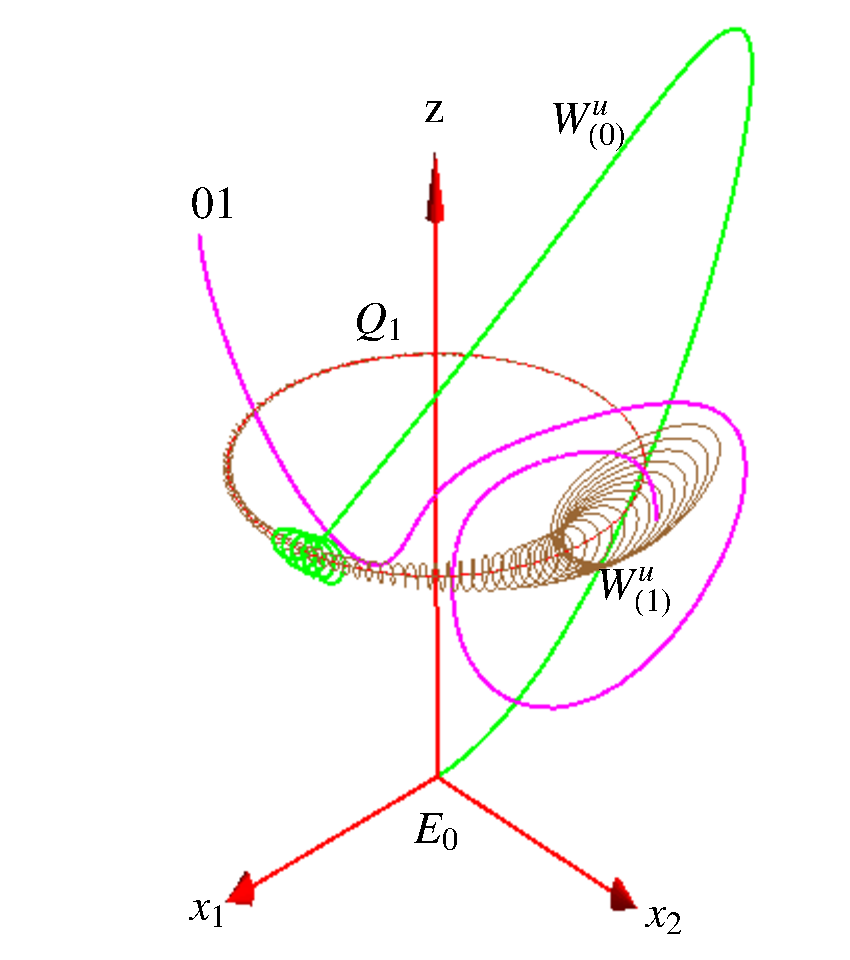
\includegraphics[width=0.35\textwidth,clip=true]
  {CLEcompact}
  \\
  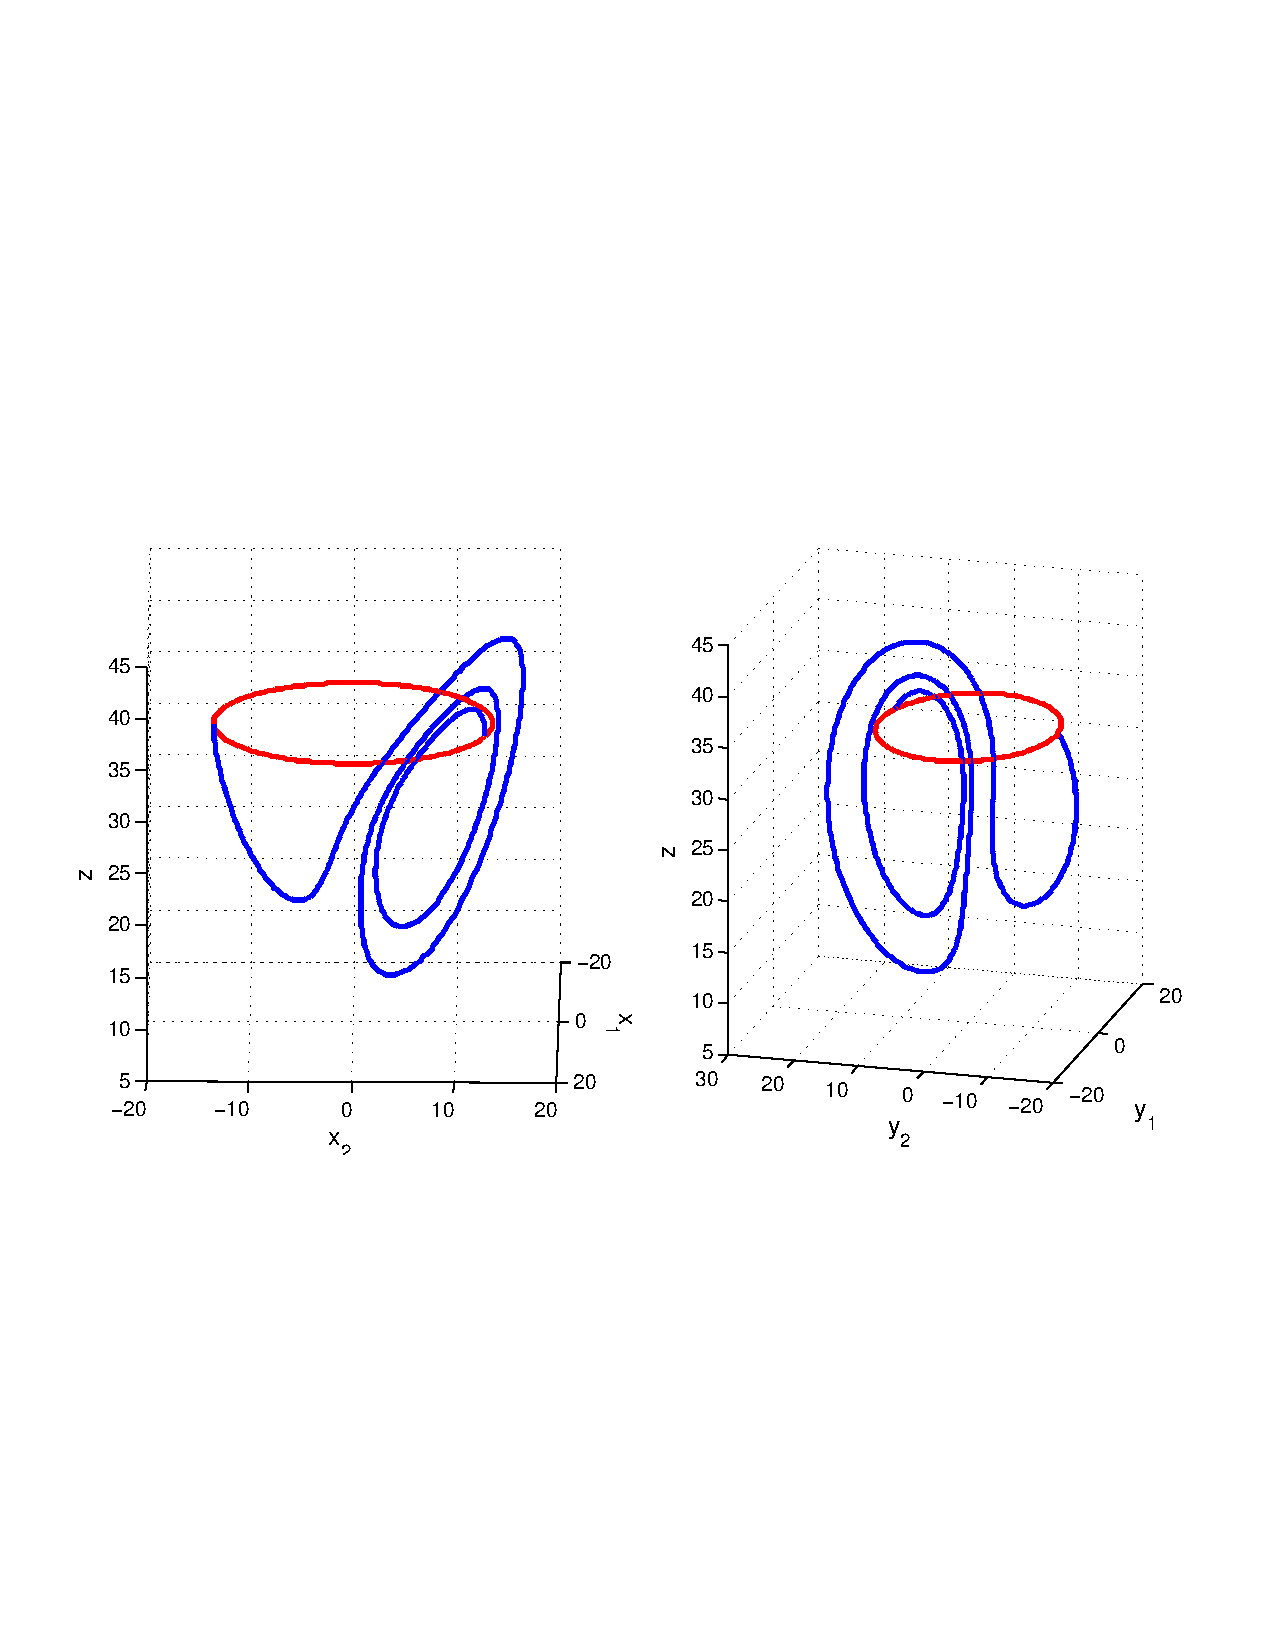
\includegraphics[width=0.7\textwidth]{CLERPO001.pdf}
\end{center}
  \caption{
\CLf:
(a) (b)
Continuous symmetry induces drifts: generic chaotic trajectory (blue);
$E_0$ \eqv;
$E_0$ unstable manifold - a cone of such (green);
$\REQV{}{0}$ \reqv\ (red);
$\REQV{}{0}$ unstable manifold, one for each point on $Q_1$ (brown);
\rpo\ \cycle{01} (purple)
(c)
    The \rpo\ \cycle{001} is shown in blue.
    The group orbit of the initial condition is shown in red.
}
\label{fig:CLERPO001}
\end{figure}

\item[2012-03-22 Predrag~~] Thanks Daniel, that clears it up - Evangelos
is vindicated. For Chaos Gang article we will need a figure like
\reffig{fig:CLERPO001}\,{(c)}, but for the purple cycle \cycle{01} in
\reffig{fig:CLERPO001}\,{(b)}, together with the (red) \reqv\
$\REQV{}{0}$. Make it pretty, at least as pretty as
\reffig{fig:CLERPO001}\,{(b)}, and \emph{small} *.pdf. Save the
program in siminos/figSrc, document it (what it is, how it works) in
siminos/figSrc/00ReadMe.txt.

Next, plot \cycle{01}  in your single slice program - I sure hope it
jumps at the far end of the slice hyperplane, and that you verify it
reaches beyond it \chartBord. Take the furthest point beyond the jump,
use it as template, do as \reffig{fig:A29-2slices} says. Either you
triumph, or you explain what is wrong with my line of thought.

Keith stopped by - is thinking, but will be out of action for next few
dates.

\item[2012-03-22 Predrag~~] To Bryce and Daniel: I think yesterday's
argument about fixing the Poincar\'e section by  minimizing the distance
\beq
\Norm{\ssp(\zeit) - \slicep)}
\ee{minDistPinc}
under time variation is wrong.  Try it out yourself.

\item[2012-03-23 Keith~~] Fixed my code for slicing, and am working on checking 2 slices; need to think about nature of edge.  Bryce, I think you and I are on the same page about running into the troublesome areas before being able to transfer from 1 slice to the other.  Have you troubleshot this and I missed it?  I will think about this and will check this while away; perhaps I am misunderstanding these discontinuities.

\end{description}
